\documentclass[a4paper,12pt]{article}
\usepackage[utf8]{inputenc}
\usepackage[T1]{fontenc}
\usepackage[serbian]{babel}
\usepackage{amsmath}
\usepackage{url}
\usepackage{hyperref}
\usepackage{listings}
\usepackage{xcolor}
\usepackage{lmodern}
\usepackage{float}   
\usepackage{subcaption}
\usepackage{float}

\usepackage{graphicx} % Required for inserting images

\lstset{
    language=Python,
    basicstyle=\ttfamily\small,
    keywordstyle=\color{blue},
    commentstyle=\color{gray}\itshape,
    stringstyle=\color{red},
    numbers=left,
    numberstyle=\tiny\color{gray},
    stepnumber=1,
    numbersep=5pt,
    showstringspaces=false,
    breaklines=true,
    frame=single,
}

\renewcommand{\figurename}{Slika}  % Change "Figure" to "Slika"
\renewcommand{\tablename}{Tabela}
\begin{document}

\begin{titlepage}
    \centering
	\begin{figure}[htbp]
    	\centering
    	
\includegraphics[width=0.4\textwidth]{logo.png}
	\end{figure}
    { Univerzitet u Beogradu \\ Matematički fakultet\par}
	
    \vfill

    {\Large \textbf{Projekat iz Računarske inteligencije}\par}

    \vspace{1cm}

    \begin{center}
    {\Large \textbf{Artistic Image Transformation}}\\
    {\Large \textbf{using Neural Style Transfer}}
    \end{center}

    \vfill

    
	
	
	\begin{tabbing}
        \hspace{10cm} \= \hspace{10cm} \kill
        \textbf{Mentor:} \>  \textbf{Studenti:} \\
        Asistent Stefan Kapunac \> Jovana Urošević 189/2021 \\
        \textbf{Profesor: } \> Smer: Informatika \\
        Vladimir Filipović \>
    \end{tabbing}
    
    \vfill

    \textbf{Datum:} 2024/25

\end{titlepage}
\newpage
\tableofcontents
\newpage
\section*{Uvod}

\emph{Neural Style Transfer} -- NST predstavlja tehniku iz domena veštačke inteligencije i dubokog učenja koja omogućava kombinovanje dve slike -- jedne sadržajne slike (npr. fotografije) i jedne stilske slike (npr. umetničkog dela) -- u novu, sintetičku sliku koja zadržava prepoznatljiv sadržaj prve slike, ali je vizuelno predstavljena u stilu druge slike. Drugim rečima, cilj je da se objekti i struktura iz originalne fotografije prikažu kao da su naslikani tehnikama i bojama izabrane umetničke slike. Ovaj problem je prvi put uspešno rešen 2015. godine algoritmom koji su predstavili Gatys i saradnici u radu \emph{“A Neural Algorithm of Artistic Style”}. Njihova metoda koristi duboku konvolutivnu neuronsku mrežu (prethodno naučenu za prepoznavanje objekata) da izvuče karakteristike (\emph{feature}) slike na više nivoa apstrakcije, i zatim definiše funkciju greške koja poredi sličnost sadržaja i stila izmeđ u kombinovane slike i originalnih slika. Optimizacijom te funkcije greške dobijamo novu sliku koja ostvaruje kompromis izmeđ u zadržavanja istog sadržaja i usvajanja tuđeg stila.

U ovom projektu implementirana je NST metoda korišćenjem unapred naučene duboke mreže VGG19 za ekstrakciju sadržajnih i stilskih karakteristika slika. Primenjena su dva pristupa za generisanje stilizovane slike:
\begin{itemize}
\item \textbf{Optimizacioni pristup (bazna metoda):} direktna optimizacija piksela slike pomoću gradijentskog optimizatora (Adam)
\item \textbf{Evolucioni pristup:} formulacija problema kao genetskog algoritma (GA) koji evoluira populaciju kandidata-slika kroz operatore selekcije, ukrštanja i mutacije. Takođe je ispitana hibridna varijanta koja kombinuje GA sa lokalnom pretragom pomoću Adam optimizatora, radi ubrzanja konvergencije.
\end{itemize}

Dokumentacija u nastavku prvo objašnjava teorijsku osnovu neuronskog prenosa stila -- ulogu konvolutivne mreže VGG19 u izdvajanju sadržaja i stila, koncept Gramove matrice za predstavljanje stila, kao i formulaciju funkcije gubitka. Zatim se detaljno opisuju implementirani pristupi, uključujuci sve relevantne parametre (optimizator Adam, podešavanja genetskog algoritma: predstavljanje jedinke, inicijalizacija populacije, selekcija, ukrštanje, mutacija, elitizam), kao i integracija lokalne gradijentske pretrage unutar GA. Na kraju se prikazuju i analiziraju rezultati eksperimenata za različite varijante algoritma i porede se performanse genetskog pristupa naspram standardnog NST optimizacionog pristupa.

\section{Neural Style Transfer -- teorijska pozadina}
\subsection{Ekstrakcija sadržaja i stila pomoću VGG19}
Ključno opažanje koje NST čini mogućim jeste da duboke konvolutivne mreže -- naučene da prepoznaju razne objekte na slikama -- uspešno izdvajaju višeslojne reprezentacije slike: niži slojevi hvataju nisko-nivojske detalje (ivice, teksture), dok viši slojevi hvataju strukturu i globalne rasporede objekata. Mreža VGG19 je duboka konvolutivna neuronska mreža sa 19 slojeva (16 konvolucija i 3 potpuno povezana sloja) koja je trenirana na velikom skupu slika (ImageNet) za klasifikaciju objekata. Ova mreža se često koristi kao \emph{feature extractor} u NST algoritmu. U ovom radu koristi se VGG19 model sa zamrznutim težinama (tj. bez daljeg učenja) za izračunavanje reprezentacija sadržaja i stila ulaznih slika.

Ulaz u VGG19 je slika dimenzija $H\times W$ piksela (sa 3 kanala boja), a izlazi konvolucija u datom sloju su tenzori (tzv. \emph{feature mape}) dimenzija $H_l\times W_l \times C_l$ za sloj $l$ (gde $C_l$ predstavlja broj filtera/kanala u tom sloju). Da bi se numerički kvantifikovali sadržaj i stil slike, biraju se odgovarajući slojevi u VGG mreži:
\begin{itemize}
\item \textbf{Sadržajni sloj:} treba da hvata strukturu i raspored objekata na slici, zanemarujući nisko-nivojske detalje. To su obično dublji slojevi mreže (jer oni zadržavaju semantičke informacije, a gube precizne teksture). U skladu sa time, kao sloj za ekstrakciju sadržaja odabran je konvolucioni sloj \texttt{block5\_conv2} mreže VGG19 (peti blok konvolucija, drugi konv. sloj), slično pristupu Gatys \emph{et al.} koji su koristili \texttt{conv4\_2} sloj VGG mreže. Izlaz ovog sloja na datoj slici predstavlja skup aktivacija $F^c_{ij}$ (gdje je $i$ indeks kanala, $j$ indeks pozicije u okviru tog kanala) koje služe kao vektor karakteristika sadržaja.

\item \textbf{Stilski slojevi:} treba da hvataju vizuelni stil slike na različitim skalama -- od lokalnih tekstura do globalnih paterna. Empirijski se pokazalo da se dobar balans dobija ako se uzima više slojeva raspoređenih kroz dubinu mreže. U ovom radu korišćeni su prvi konvolucioni slojevi iz svakog od pet konvolucionih blokova VGG19: \texttt{block1\_conv1}, \texttt{block2\_conv1}, \texttt{block3\_conv1}, \texttt{block4\_conv1} i \texttt{block5\_conv1}. Ovi slojevi obezbeđuju da se stil posmatra na više nivoa detalja -- od najnižeg (prvi sloj hvata osnovne šare) do najvišeg (npr. \texttt{block5\_conv1} hvata globalnije rasporede tekstura).
\end{itemize}
Nakon što se kroz VGG19 propagira slika, sa ovih odabranih slojeva možemo pročitati dve vrste podataka: (1) skup aktivacija neurona sadržajnog sloja (koji se koristiti za poređenje sadržaja), i (2) skup aktivacija sa svakog stilskog sloja (koji će se dalje obraditi kako bi se dobila reprezentacija stila).

\subsection{Gramova matrica kao reprezentacija stila}
Da bi se numerički opisao stil slike, potrebno je metrikom obuhvatiti teksturne karakteristike koje nisu zavisne od tačne pozicije na slici, već od statističkih raspodela i korelacija vizuelnih elemenata. Gatys \emph{et al.} su uveli koncept \textbf{Gramove matrice} kao reprezentacije stila slike. Gramova matrica kodira korelaciju izmeđ u aktivacija kanala u jednom konvolucionom sloju. Za dati sloj $l$ sa $C_l$ kanala (feature mapa), prvo se oblikuje njegov izlaz $F^l$ u dvodimenzioni oblik $C_l \times N_l$, gde je $N_l = H_l \times W_l$ broj pozicija (piksel-lokacija) unutar svih feature mapa tog sloja. Dakle, svaki od $C_l$ kanala postaje vektor dužine $N_l$ koji sadrži aktivacije tog filtera preko cele slike. Vektori se označavaju sa $\mathbf{f}1, \mathbf{f}2, \dots, \mathbf{f}{C_l}$. Tada je \textbf{Gramova matrica} sloja $l$ definisana kao:
\[
G^l = F^l (F^l)^{T},
\]
odnosno element $G^l_{ij}$ predstavlja skalarni proizvod između vektora kanala $i$ i kanala $j$:
\[
G^l_{ij} = f_i \cdot f_j = \sum_{k=1}^{N_l} f_{ik} f_{jk}.
\]

Gramova matrica je dimenzija $C_l \times C_l$ i meri u kojoj meri su filter $i$ i filter $j$ istovremeno aktivni na istim prostornim lokacijama slike. Intuitivno, ova korelacija hvata informaciju o teksturi: npr. ako su određeni kanali (koji detektuju specifične oblike ili šare) često zajedno aktivni, to ukazuje na prisustvo određene stilske karakteristike u slici.

Za svaku sliku se može izračunati Gramova matrica za svaki od izabranih stilskih slojeva. Da bi stil sintetičke slike bio sličan stilskoj slici, njihove Gramove matrice treba da budu slične. S druge strane, sadržaj slike se poredi direktno putem vrednosti aktivacija u sadržajnom sloju (jer one nose informaciju o rasporedu objekata). 

\subsection{Funkcija gubitka za NST}
Algoritam neuronskog prenosa stila formuliše generisanje stilizovane slike kao optimizacioni problem. Definiše se \textbf{funkcija gubitka} (funkcija greške) koja meri odstupanje trenutno generisane slike od željenog sadržaja i stila, i zatim se ta slika iterativno optimizuje (pomocu gradijentnog spusta ili drugog optimizacionog metoda) da minimizira zadati gubitak.

Ukupni gubitak obuhvata dva dela:
\[
L_{\text{ukupno}}(\text{generisana slika}) 
= \alpha \, L_{\text{sadržaj}} + \beta \, L_{\text{stil}},
\]
gde su $\alpha$ i $\beta$ hiperparametri (\emph{težinski faktori}) kojima se podešava relativni značaj sadržaja naspram stila.  

Drugim rečima, $L_{\text{sadržaj}}$ meri koliko generisana slika odstupa od sadržajne slike, a $L_{\text{stil}}$ meri odstupanje od stilske slike; parametri $\alpha$ i $\beta$ (poznati i kao \emph{content weight} i \emph{style weight}) balansiraju ova dva kriterijuma.

\paragraph{Gubitak sadržaja.} 
Da bi se kvantifikovala sadržajna razlika, korišćeno je predstavljene karakteristike iz odabranog sadržajnog sloja mreže. 
Neka je $\mathbf{P}$ originalna sadržajna slika, $\mathbf{X}$ trenutna generisana slika, a $F^l(\mathbf{X})$ označava vektor 
(tj. skup aktivacija svih neurona) sadržajnog sloja $l$ za sliku $\mathbf{X}$. 
Tada je funkcija gubitka sadržaja definisana kao srednja kvadratna greška (\emph{mean squared error}, MSE) između 
odgovarajućih aktivacija za generisanu i originalnu sliku:
\[
L_{\text{sadržaj}}(\mathbf{X}, \mathbf{P}) 
= \frac{1}{2} \sum_i \sum_j \Big( F^l_{ij}(\mathbf{X}) - F^l_{ij}(\mathbf{P}) \Big)^2.
\]

U praksi se suma može normalizovati (npr. podeliti sa brojem elemenata) kako bi veličina ovog gubitka bila u sličnom 
opsegu kao gubitak stila; alternativno, razlika u opsegu se reguliše faktorima $\alpha, \beta$.


\paragraph{Gubitak stila.} 
Za poređenje stila između generisane slike $\mathbf{X}$ i stilske slike $\mathbf{A}$, koristi se Gramova matrica za svaki od $L$ odabranih stilskih slojeva. 
Neka $G^l(\mathbf{X})$ označava Gramovu matricu $l$-tog sloja za sliku $\mathbf{X}$, a $G^l(\mathbf{A})$ za stilsku sliku. 
Gubitak stila definiše se kao kvadratna greška između ovih matrica, sumirana preko svih stilskih slojeva:
\[
L_{\text{stil}}(\mathbf{X}, \mathbf{A}) 
= \sum_{l=1}^{L} w_l \sum_i \sum_j \Big( G^l_{ij}(\mathbf{X}) - G^l_{ij}(\mathbf{A}) \Big)^2.
\]

Ovde $w_l$ mogu biti težine kojima se može dati veći značaj određenim slojevima stila; 
često se uzima da su svi jednaki ili da se normiraju obrnuto proporcionalno broju neurona sloja, 
tako da svaki sloj podjednako doprinese. 
U ovom projektu, radi jednostavnosti korišćene su jednake težine po sloju 
(implementacija koristi prosečnu vrednost razlike umesto sume, što je ekvivalentno uniformnom ponderisanju).

\paragraph{Optimizacija slike.} Nakon definisanja $L_{\text{ukupno}}(\mathbf{X})$, problem prenosa stila svodi se na nalaženje slike $\mathbf{X}$ koja minimizuje ovu funkciju. Važno je naglasiti da se prilikom ove optimizacije \textbf{parametri VGG mreže ne menjaju} -- ona služi samo kao fiksni mehanizam za ekstrakciju karakteristika. Mijenjaju se \textbf{direktno pikseli} generisane slike $\mathbf{X}$. U startu, $\mathbf{X}$ se može inicijalizovati slučajno ili nekom od ulaznih slika. Gatys \emph{et al.} su inicijalizovali šumom, ali je kasnije primećeno da inicijalizacija na sadržajnu sliku ubrzava konvergenciju i često daje bolja početna svojstva, pa sam i u ovom projektu koristila sadržajnu sliku kao polaznu tačku sintetičke slike.

Optimizacija se može izvršiti standardnim algoritmima gradijentnog spusta. Originalni rad je koristio L-BFGS optimizator, dok je u ovom projektu korišćen \emph{Adam} optimizator (varijanta stohastičkog gradijentnog spusta sa adaptivnim korakom učenja). Gradijent funkcije gubitka u odnosu na piksele slike $\nabla_{\mathbf{X}} L_{\text{ukupno}}$ možemo izračunati automatskom diferencijacijom kroz mrežu (koristeći \texttt{tf.GradientTape} u TensorFlow). Zatim se pikseli slike iterativno ažuriraju u smeru opadajućeg gradijenta.

U mom slučaju, faktori za balansiranje uzeti su $\alpha = 10^{4}$ (za sadržaj) i $\beta = 10^{-2}$ (za stil). 
Ovim je osigurano da generisana slika zadrži osnovne oblike i strukturu sadržajne slike, dok stil 
(koji je po samoj meri definisan drugačije) ne dominira previše. 
Ovakav odnos težina je standardan i dokazano efikasan u literaturi o prenosu stila . 
Nakon nekoliko stotina do hiljadu iteracija optimizacije, funkcija gubitka tipično konvergira ka nekoj minimalnoj vrednosti, 
a dobijena slika vizuelno predstavlja dobru kombinaciju sadržaja i stila.

\newpage
\section{Implementacija i eksperimenti}
U ovom poglavlju opisani su implementacioni detalji i rezultati dva pristupa generisanju stilizovane slike: baznog pristupa optimizacije slike Adam optimizatorom i evolutivnog pristupa korišćenjem genetskog algoritma. Eksperimenti su sprovedeni nad istim ulaznim slikama (jedna sadržajna i jedna stilska), pri čemu su hiperparametri NST gubitka (odabrani slojevi, tezinski faktori sadržaja i stila) ostali fiksni kako bi se omogućilo fer poređenje metoda. Korišćena je funkcija za ekstrakciju karakteristika (\texttt{StyleContentExtractor}) opisana u prethodnom poglavlju, koja internom VGG19 modelu prosleđuje sliku i vraća rečnike sa ključevima \texttt{'content'} i \texttt{'style'}: sadržajni vektor (aktivacije sloja \texttt{block5\_conv2}) i Gram-matrice za stil (za slojeve \texttt{block1\_conv1} ... \texttt{block5\_conv1}). Slede detaljno prikazani postupak bazne optimizacije, a potom genetski algoritam i njegove varijacije.

\subsection{Bazni pristup — optimizacija pomoću ručno implementiranog Adam algoritma}
Bazni NST pristup tretira generisanu sliku kao skup parametara koje treba optimizovati minimizacijom definisane funkcije gubitka. Implementacija je izvedena u TensorFlow okruženju, pri čemu je Adam algoritam \emph{ručno} implementiran korišćenjem pokretnih sredina prvog i drugog momenta gradijenta. Inicijalna generisana slika $\mathbf{X}$ postavljena je jednaka sadržajnoj slici (pretvorena u tenzor odgovarajućih dimenzija i normalizovana na opseg vrednosti $[0,1]$).

U svakoj iteraciji koristi se \texttt{GradientTape} za računanje gradijenta $\nabla_{\mathbf{X}} L_{\text{ukupno}}$, nakon čega se ažuriraju momenati $m$ i $v$:
\[
m \leftarrow \beta_1 m + (1-\beta_1)\nabla_{\mathbf{X}} L, \qquad
v \leftarrow \beta_2 v + (1-\beta_2)\big(\nabla_{\mathbf{X}} L\big)^2,
\]
a zatim se primenjuju bias-korekcije
\[
\hat m = \frac{m}{1-\beta_1^t}, \qquad
\hat v = \frac{v}{1-\beta_2^t},
\]
i ažuriranje slike
\[
\mathbf{X} \leftarrow \mathbf{X} - \alpha \frac{\hat m}{\sqrt{\hat v}+\varepsilon}.
\]
Nakon svakog koraka vrednosti piksela se projekcijom vraćaju u opseg $[0,1]$.

Korišćeni hiperparametri bili su: stopa učenja $\alpha=0.02$, $\beta_1=0.99$, $\beta_2=0.999$ i numerički stabilizator $\varepsilon=10^{-1}$. Izvedeno je ukupno 1000 koraka optimizacije, organizovanih u 10 epoha po 100 koraka radi preglednosti izlaza. Na kraju svake epohe prikazivana je trenutna slika i ispisivana vrednost ukupnog gubitka.

Nakon 1000 iteracija dobijena je \textbf{konačna stilizovana slika} visokog kvaliteta. Ukupni gubitak opao je na približno $1.2818\times 10^{7}$, što je višestruko niže u odnosu na početnu vrednost i demonstrira efikasnost direktne gradijentne optimizacije u usklađivanju sadržajnih i stilskih karakteristika. Vreme izvršavanja bilo je oko \textbf{23.3 s}, što odražava efikasnost TensorFlow implementacije na GPU-u za 1000 koraka optimizacije.

Vizuelno, rezultat zadržava glavne oblike i raspored iz originalne fotografije, dok preuzima teksturu, paletu boja i poteze „četkice” iz umetničke slike. Na Slici prikazan je primer rezultata NST optimizacije za jednu ulaznu kombinaciju.


\begin{figure}[h]
\centering
\begin{minipage}{0.32\textwidth}
    \centering
    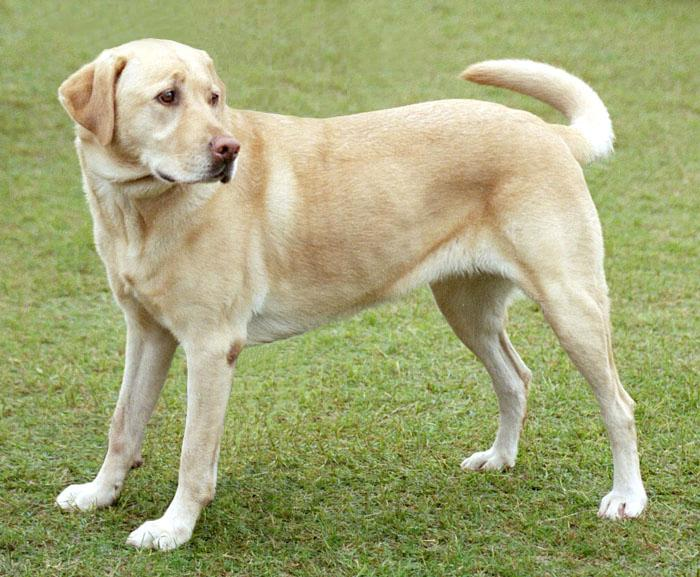
\includegraphics[width=\linewidth]{content_image.jpg}
    {Sadržajna slika}
\end{minipage}
\hfill
\begin{minipage}{0.32\textwidth}
    \centering
    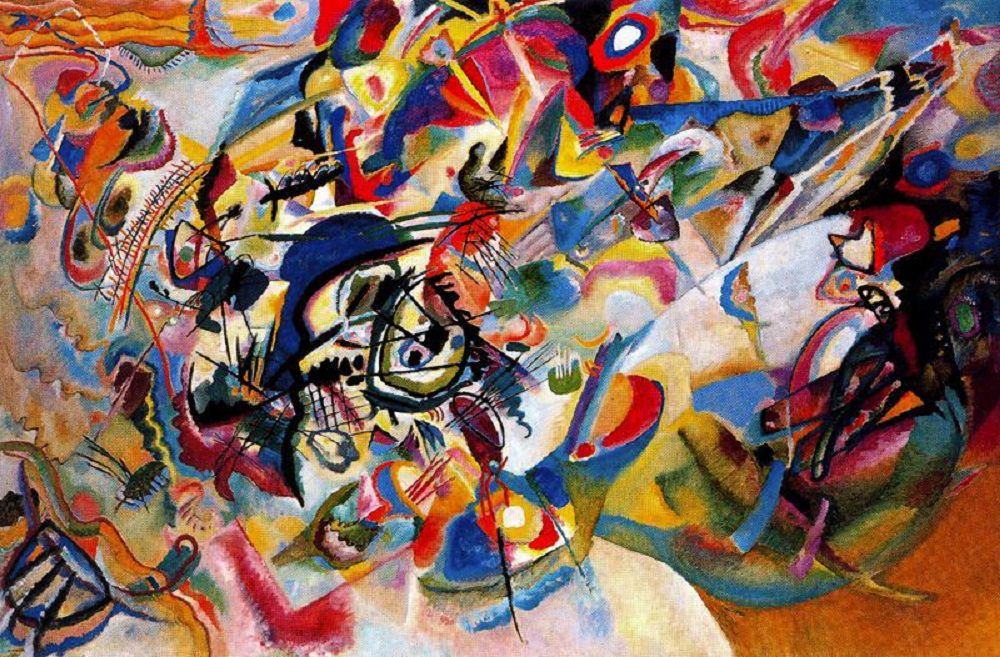
\includegraphics[width=\linewidth]{style_image.jpg}
    {Stilska slika}
\end{minipage}
\hfill
\begin{minipage}{0.32\textwidth}
    \centering
    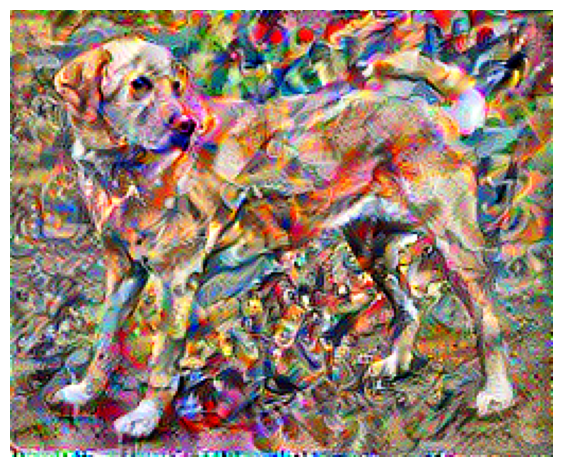
\includegraphics[width=\linewidth]{adam.png}
    {Stilizovana slika}
\end{minipage}
\end{figure}

\subsection{Evolucioni pristup -- genetski algoritam}
Nasuprot direktnom optimizovanju jedne slike, u ovom pristupu se evoluira populacija više slika-kandidata korišćenjem principa evolucije: selekcije najboljih, rekombinacije njihovih „gena“ (piksela) i mutacija (nasumičnih promena). Ideja je da, i bez eksplicitnog korišćenja gradijenata, populacija vremenom evoluira stilizovanu sliku minimizujući NST gubitak. Genetski algoritmi se često primenjuju kod optimizacionih problema u kojima je prostor pretrage diskretan ili gradijent nije dostupan; ovde je cilj ispitati koliko dobro GA može da se nosi sa kontinuiranim, visokodimenzionalnim problemom kakav je stilizacija slike i da li može dostići kvalitet rešenja koji postižu gradijentske metode.

\subsubsection{Reprezentacija jedinke i inicijalizacija populacije}
U implementaciji, definisana je klasa \texttt{Individual} koja sadrži sve potrebne informacije za jednu jedinku (kandidatsku sliku) i metode za obračun njene prilagođenosti (fitness). Svaka jedinka ima atribut \texttt{code} koji je tenzor dimenzije $1\times H \times W \times 3$ (tj. slikovni podaci u formatu odgovarajućem VGG modelu, uključujući batch dimenziju od 1). Na početku evolucije, populacija od $N$ jedinki se kreira inicijalizacijom svih \texttt{code} tenzora istom sadržajnom slikom uz dodatak male slučajne buke. Konkretnije, ako je $\mathbf{C}$ tenzor sadržajne slike (normalizovan na opseg $[0,1]$), svaka jedinka dobija $\mathbf{X}_0 = \mathbf{C} + \mathcal{N}(0, 0.05)$, gde je $\mathcal{N}(0,0.05)$ gausov šum standardne devijacije 0.05 (5\% intenziteta). Zatim se vrednosti piksela clipping-om ograničavaju u $[0,1]$. Ovakva inicijalizacija populacije osigurava da sve jedinke kreću iz stanja bliskog sadržajnoj slici (dakle, populacija inicijalno sadrži slike koje su veoma slične originalnoj fotografiji, uz jedva primetne šumne varijacije). 

Svaka jedinka odmah pri kreiranju izračunava svoju vrednost \textbf{fitness} funkcije, što je zapravo samo negirana ukupna NST funkcija gubitka:
\[
\text{fitness} = -L_{\text{ukupno}} = -(\alpha L_{\text{sadržaj}} + \beta L_{\text{stil}})
\]
Korišćen je negativan gubitak zato što se u genetskom algoritmu maksimizira fitness (bolje jedinke imaju veći fitness), dok je cilj minimizacija stila/sadržaja gubitka. Dakle, jedinka sa nižim NST gubitkom imaće veći (manje negativan) fitness i biće favorizovana u selekciji. U momentu inicijalizacije, fitness svih jedinki će biti relativno sličan (jer su im slike slične, sve bliske sadržajnoj slici). Obračun fitnessa realizovan je metodom \texttt{calc\_fitness()} unutar klase \texttt{Individual}, koja koristi već definisani ekstraktor karakteristika: propagira jedinkinu sliku kroz VGG19 i računa $L_{\text{sadržaj}}$ i $L_{\text{stil}}$ sa fiksnim metrikama kao gore. U implementaciji su korišćene iste vrednosti $\alpha=10^4$ i $\beta=10^{-2}$ kao i u baznoj metodi, tako da je poređenje rezultata konzistentno.

\subsubsection{Selekcija}
Genetski algoritam iterativno evoluira populaciju kroz generacije. U svakoj generaciji potrebna je procedura \textbf{selekcije roditelja} za reprodukciju (ukrštanje). Odabran je stohastički postupak selekcije poznat kao \emph{turnirska selekcija} (engl. \emph{tournament selection}). Turnirska selekcija funkcioniše tako što se nasumično iz populacije izabere $k$ jedinki (bez obzira na njihov fitness), i zatim se od njih odabere najbolja (ona sa najvišim fitnessom) kao roditelj. U algoritmu korišćena je veličina turnira $k=3$, tj. biraju se tri kandidata pa uzimamo najboljeg od njih kao roditelja. Ovaj postupak ima prednost da ne zahteva proporcionalne verovatnoće niti sortiranje cele populacije za svako biranje, a ipak daje prednost boljim jedinkama uz očuvanje raznolikosti (uvek postoji šansa da i slabija jedinka bude izvučena u turnir, pogotovo ako je populacija velika). Implementirano je metodom \texttt{selection()} u klasi GA, koja vraća jednu izabranu jedinku. Za potrebe ukrštanja, biramo dva roditelja pozivajući selekciju dva puta (drugi put pazimo da drugi roditelj nije identičan prvom, kako ne bismo ukrštali jedinku sa samom sobom).

\subsubsection{Ukrštanje}
Operator \textbf{ukrštanja} (\emph{crossover}) kombinuje informacije dve roditeljske jedinke da bi proizveo novo rešenje (dva deteta). Postoji mnogo mogućih načina da se slike "ukrste". Ovde je implementiran jednostavan postupak \emph{jedne tačke ukrštanja} inspirisan genetikom, gde se slike podele na dva dela duž jedne prostorne ose, i delovi zamene između roditelja. Konkretnije, nasumično se odredi horizontalna linija kroz sliku (odnosno indeks reda piksela) na poziciji $y_{\text{split}}$ uniformno u opsegu $[0, H]$. Tada se konstrukcija dece radi tako što prvo dete dobija piksele roditelja~1 iz svih redova iznad te linije, a piksele roditelja~2 ispod te linije; za drugo dete obrnuto (gornji deo od roditelja~2, donji od roditelja~1). 

U kodu, to je izvedeno kreiranjem binarne maske veličine slike: gornji deo maske čine jedinice, donji deo nule (ili obratno), i zatim:
\[
\text{dete}_1 = \text{roditelj}_1 \odot \text{maska} + \text{roditelj}_2 \odot (1-\text{maska}),
\]
\[
\text{dete}_2 = \text{roditelj}_2 \odot \text{maska} + \text{roditelj}_1 \odot (1-\text{maska}),
\]
gde je $\odot$ pikselska (Hadamardova) multiplikacija. Ovim svako dete dobija kompletan gornji segment od jednog roditelja i kompletan donji segment od drugog. Dobijena tenzorska reprezentacija se zatim koristi za kreiranje novih \texttt{Individual} objekata (koji će odmah izračunati svoj fitness).

Ukrštanje se primenjuje na parove roditelja sve dok se ne dobije potreban broj novih jedinki da popune populaciju sledeće generacije. U ovoj implementaciji korišćena je veličina populacije $N=20$. Takođe je uveden \textbf{elitizam}: najboljih $E$ jedinki iz prethodne generacije se direktno prenose u sledeću generaciju nepromenjeni (tzv. \emph{elitna populacija}), a ostatak $N-E$ jedinki se dobija ukrštanjem. Postavljeno je  $E=2$, što znači da 2 najbolja rešenja uvek preživljavaju netaknuta u narednu generaciju. Elitizam obezbeđuje monoton rast kvaliteta najbolje jedinke ili barem očuvanje trenutno najboljeg pronađenog rešenja tokom evolucije (sprečava regresiju zbog stohastičkih operacija).

\subsubsection{Mutacija}
Operator \textbf{mutacije} uvodi nasumične promene kod jedinki (dece) radi diverzifikacije genetskog materijala i izlaska iz eventualnih lokalnih optimuma. U kontekstu slike, mutacija bi mogla biti nasumična perturbacija piksela. Međutim, sa znanjem o ovom problemu, implementirane su dve vrste mutacija -- jednu vođenu gradijentom, i drugu nasumičnu, te se nasumično bira koja se primenjuje na dato dete. Na ovaj način kombinovana je \emph{eksploatacija} (fino unapređivanje postojećih rešenja) i \emph{eksploracija} (istraživanje novih kombinacija stila i sadržaja).


U kodu se, za svako novodobijeno dete (posle ukrštanja) baca novčić (50\% šanse) da bi se odlučio tip mutacije:
\begin{itemize}
\item \textbf{Mutacija gradijentom:} Sa verovatnoćom $p = 0.4$ (tj. parametar \texttt{mutation\_rate}) primenjuje se jedan korak gradijentskog spuštanja na slici deteta u cilju smanjenja NST gubitka. U suprotnom (sa verovatnoćom $0.6$) ne radi se ništa na toj jedinki. Dakle, ova mutacija koristi \textbf{informaciju gradijenta} kako bi potencijalno popravila dete posle ukrštanja. Implementirano je metodom \texttt{mutate\_with\_gradient(step\_size, mutation\_rate)} unutar klase \texttt{Individual}: koristi se \texttt{tf.GradientTape} da izračuna gradijent $\nabla_{\mathbf{X}} L$ za sliku date jedinke; zatim se taj gradijent doda slici skaliran malim korakom $\eta$ (hiperparametar \texttt{step\_size}, ovde $\eta=0.3$). Ovaj postupak se obavi samo ako se generiše slučajan broj $< \texttt{mutation\_rate}$ (inače se preskače), čime se ostvaruje gore pomenuta verovatnoća primene mutacije. Nakon eventualne gradijentske promene, pikseli se ograniče u $[0,1]$.
\item \textbf{Slučajna mutacija:} Ako je odaberana ova mutacija (u 50\% slučajeva), dete se modifikuje bez korišćenja gradijenata, čisto nasumično ali na način vođen problemom. U implementaciji je urađeno sledeće: nasumično je izabrano da li će se dete "povući" malo ka stilskoj ili ka sadržajnoj slici (sa po 50\% verovatnoće). Zatim izračunato
\[
\mathbf{X}' = (1-\alpha)\mathbf{X} + \alpha \mathbf{T} + \mathcal{N}(0,\sigma^2),
\]
gde je $\mathbf{X}$ originalna slika deteta, $\mathbf{T}$ je ciljana slika za povlačenje (što je ili $\mathbf{C}$ sadržajna ili $\mathbf{A}$ stilska), $\alpha=0.1$ je mali faktor mešanja od 10\%, a $\mathcal{N}(0,\sigma^2)$ je dodatni šum. Parametar $\sigma$ (standardna devijacija šuma) je vezan za \texttt{mutation\_rate}, konkretno $\sigma = \texttt{mutation\_rate} = 0.4$. To znači da se dodaje relativno umeren nivo slučajnog šuma. Ideja ovog postupka je da se dete pomeri blago ka nekom od poznatih polova (sadržaju ili stilu) i doda se buka da bi se uneli novi detalji. Nakon ove operacije takođe se radi clipping piksela u $[0,1]$.
\end{itemize}

Svako dete prolazi kroz jednu od ove dve mutacije (ili ostane nepromenjeno ako u okviru gradijent-mutacije nije ispunjen uslov verovatnoće). Nakon mutacije, ako je dete modifikovano (njegov tenzor slike promenjen), ponovo se izračuna fitness (jer se sada slika promenila). U ovo implementaciji, otprilike polovina dece dobije gradijentsku mutaciju, a polovina stohastičku, što je ispalo efektno u praksi da se održi ravnoteža između malih poboljšanja najboljih jedinki i istraživanja novih kombinacija stil-sadržaj.

\subsubsection{Evolucija kroz generacije i rezultati osnovnog GA}
Kompletan genetski algoritam sastoji se od ponavljanja sledećeg procesa za zadati broj generacija:
\begin{enumerate}
\item Populacija se sortira po fitnessu opadajuće (najbolji prvi).
\item Proverava se i sačuva globalno najbolji ako je nadmašio prethodnog (ovaj globalni najbolji služi za završni rezultat).
\item Ispisuju se informacije o trenutnoj generaciji: indeks generacije, najbolji fitness, i prikazuje se slika najbolje jedinke radi praćenja (u toku eksperimenta).
\item Formira se nova populacija: prvo se kopira $E$ najboljih (elitizam), a zatim se za preostalih $N-E$ mesta biraju roditelji i prave deca ukrštanjem + mutacijom, kako je gore opisano.
\item Novodobijena populacija postaje tekuća populacija za sledeću generaciju.
\end{enumerate}

Za parametre genetskog algoritma odabrano je:
\begin{itemize}
\item Veličina populacije $N = 20$,
\item Elitizam $E = 2$,
\item Turnir za selekciju veličine 3,
\item Verovatnoća (stopa) mutacije \texttt{mutation\_rate} = 0.4,
\item Broj generacija: 50.
\end{itemize}

Prvo je izvršen eksperiment \textbf{bez lokalne pretrage} (čist GA kako je gore opisano, koji već sadrži izvesnu gradijentnu mutaciju ali samo u jednom koraku i uslovno). Ova varijanta dalje se označava sa \texttt{apply\_local\_to = None} u smislu hibridnog modela (što znači da dodatna Adam optimizacija nije uključena tokom evolucije). Nakon 50 generacija, posmatran je najbolji dobijeni rezultat i vreme izvođenja.

Rezultati su pokazali da \textbf{osnovni genetski algoritam} nije uspeo da postigne naročito nisku vrednost NST gubitka. Najbolja jedinka posle 50 generacija imala je fitness $\approx -9.2524 \times 10^9$, što odgovara ukupnom gubitku od oko $9.25 \times 10^9$. Ova vrednost je višestruko veća (lošija) od one koju je postigao bazni gradijentski pristup (koji je bio $1.28 \times 10^7$). Iako se fitness jeste popravljao kroz generacije (početni fitness jedinki bio je oko $-1.02 \times 10^{10}$ za populaciju inicijalizovanu na sadržajnu sliku), tempo napretka bio je veoma spor i činilo se da je posle $\sim 50$ generacija dostignuta plato faza bez dramatičnog poboljšanja. Kriva najboljeg fitnessa po generacijama (Slika 2) pokazuje blago povećanje na početku i dug period stagnacije. Razlog za ovako sporo unapređenje jeste to što genetski operatori, iako su unosili promene, nisu dovoljno efikasno podešavali piksele slike prema minimizaciji složene funkcije gubitka. Prostor rešenja (svi mogući pikseli slike) ogroman je i vrlo visoke dimenzionalnosti (slika od 256x256 piksela ima preko 65k parametara * 3 kanala), te nasumične mutacije i prost ukršaj ne mogu lako da pronađu fine, koordinisane promene potrebne da se smanji stilski gubitak. Čak i sa gradijentnom mutacijom od jednog koraka, ta količina bila je očigledno nedovoljna da značajno pogura rešenja ka optimumu.

\begin{figure}[h]
\centering
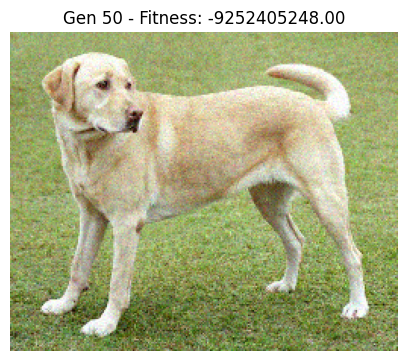
\includegraphics[width=0.7\textwidth]{ga_none.png}
\caption{Ovo je rezultat nakon 50 generacija}
\label{fig:primer_slika}
\end{figure}


Vreme izvršavanja osnovnog GA (50 generacija, populacija 20) iznosilo je oko \textbf{118.13 sekundi}. Ovo je otprilike 5 puta duže od bazne Adam optimizacije, a rezultat je bio slabijeg kvaliteta. Na osnovu ovih rezultata može se zaključiti da čisti evolucioni pristup nije konkurentan gradijentskom za problem NST, ali je zatim ispitana mogućnost da se ta razlika umanji ubacivanjem snažnije lokalne pretrage (više gradijentnih koraka) tokom GA evolucije.

\begin{figure}[h]
\centering
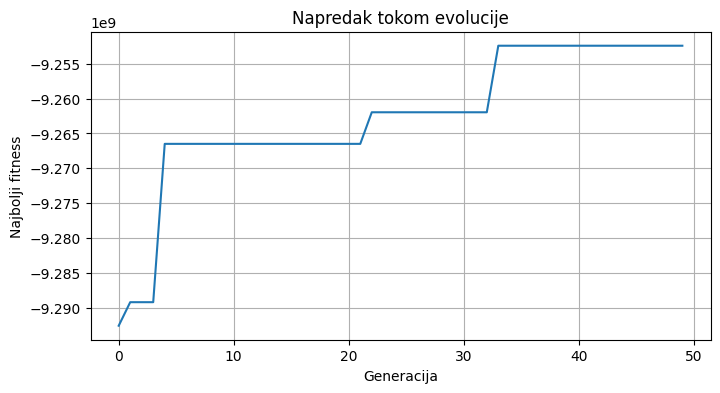
\includegraphics[width=0.8\textwidth]{fitness_curve_none.png}
\caption{Napredak najbolje jedinke tokom evolucije za osnovni genetski algoritam (bez dodatne lokalne pretrage). Prikazana je promena najboljeg fitnessa kroz 50 generacija. Uočava se vrlo sporo povećanje fitnessa (smanjenje gubitka) i približno stagniranje nakon određenog broja generacija.}
\end{figure}


\subsection{Hibridni genetski algoritam sa lokalnom Adam pretragom}
Jasno je da su gradijentske metode višestruko efikasnije u ovom problemu; stoga je implementiran \textbf{hibridni pristup} koji kombinuje GA sa periodičnom lokalnom optimizacijom jedinki pomoću Adam optimizatora. Ovakva kombinacija je poznata kao \emph{memetički algoritam} u literaturi (GA uz lokalnu pretragu) i cilj joj je da spoji globalno pretraživanje (populacioni GA koji može da istražuje različita rešenja) sa brzim lokalnim usavršavanjem rešenja (gradijent).

Hibridni algoritam je u osnovi isti GA kao gore, ali nakon formiranja nove generacije (nakon ukrštanja i mutacija), dodaje se dodatni korak:
\begin{itemize}
\item Za izvesni skup jedinki iz nove populacije (npr. najbolje ili sve), pokreće se nekoliko iteracija Adam optimizacije njihovog koda (slike) da bi se dodatno popravile. Konkretno, definisana je funkcija \texttt{local\_search(individual)} koja na datoj jedinki izvršava $m$ koraka gradijentnog spuštanja (koristeći punu NST funkciju gubitka i iste $\alpha, \beta$ kao pre). Koristi se \texttt{tf.keras.optimizers.Adam} sa određenom lokalnom stopom učenja $\eta_{\text{lokalno}}$ i izvodi $m$ iteracija ažuriranja tenzora slike unutar \texttt{GradientTape} petlje. Nakon ovih iteracija ponovo se računa fitness jedinke.
\item Ova lokalna pretraga može se primeniti ili \textbf{samo na elitne jedinke} (\texttt{apply\_local\_to="elite"} opcija) ili \textbf{na sve jedinke populacije} (\texttt{apply\_local\_to="all"}), ili se u potpunosti isključuje (\texttt{None}, što je slučaj osnovnog GA).
\end{itemize}

U eksperimentima su ispitana oba pristupa (\texttt{"elite"} i \texttt{"all"}) za dve različite vrednosti lokalne stope učenja $\eta_{\text{lokalno}}$: jednu vrlo malu ($0.002$) i jednu relativno veću ($0.2$), a dodatno i jednu srednju vrednost ($0.02$) za elitni slučaj. Broj lokalnih koraka postavljen je na $m=2$ (dakle, posle svake generacije svaka odabrana jedinka bude poboljšana sa samo dva koraka Adama). Ideja je bila da sa malim brojem lokalnih koraka ne remeti previše GA dinamiku, već da se da blagi podsticaj najboljima, dok je broj $m$ moguće povećati po potrebi (ali to značajno uvećava trošak računanja).

Za $\eta_{\text{lokalno}} = 0.002$ (vrlo konzervativno učenje), očekivalo se da lokalna pretraga pravi male pomake jedinki ka nižem gubitku, praktično fine-tuning. Za $\eta_{\text{lokalno}} = 0.2$ (agresivnije), lokalni koraci mogli bi značajno promeniti slike (potencijalno i degradirati neke, ako preteraju, ali i brzo unaprediti ako su na pravom tragu).

Evolucija je pokrenuta sa ovim podešavanjima i posmatrano je ponašanje:

\paragraph{Rezultati za $\eta_{\text{lokalno}} = 0.002$:}
\begin{itemize}
\item \textbf{Hibrid (elite):} Lokalna pretraga se primenjuje samo na najbolje 2 jedinke svake generacije. Najbolji postignuti fitness posle 50 generacija bio je \boldmath$-1.5167 \times 10^8$\unboldmath, što odgovara ukupnom gubitku $\sim 1.5167\times10^8$. Ovo je drastično poboljšanje u odnosu na osnovni GA (skoro dva reda veličine manji gubitak), ali i dalje oko 12 puta veći gubitak nego kod baznog Adam pristupa. Vreme izvršavanja bilo je \textbf{140.72 sekunde}, nešto duže od osnovnog GA, što se i očekivalo jer se dodaje dodatni račun (2 Adam koraka po generaciji na 2 jedinke).
\item \textbf{Hibrid (all):} Lokalna pretraga na svim jedinkama populacije (svih 20) posle svake generacije. Najbolji fitness na kraju bio je \boldmath$-1.4965 \times 10^8$\unboldmath; (ukupni gubitak $\sim 1.4965\times10^8$). Ovo je vrlo slično rezultatu sa elitnom pretragom (čak blago bolje, ali razlika od $0.02\times10^8$ je zanemarljiva spram apsolutne veličine). Vreme izvršavanja, međutim, skočilo je na \textbf{308.22 sekundi} što je preko dvostruko sporije (logično, jer se rade 2 koraka optimizacije na 20 jedinki = 40 optimizacija vs 4 optimizacije u elitnom slučaju, pa je time $\sim$10x veći dodatni teret po generaciji).
\end{itemize}
\textbf{Ključni uvid:} Za malu lokalnu stopu 0.002, grafik promene fitnessa po generacijama ispao je gotovo \textbf{identičan} za strategije "elite" i "all". U obe varijante, fitness se značajno brže popravljao nego u slučaju bez lokalne pretrage. Već tokom prvih 5--10 generacija najbolji fitness je pao ispod $-10^9$, zatim ispod $-10^8$, i približio se konačno oko $1.5\times10^8$. Krive su bile skoro poklopljene, što implicira da dodavanje lokalne pretrage na svakom članu populacije nije donelo bolji najbolji rezultat od fokusiranja samo na najbolje. Razlog tome može biti što kod male stope učenja, najveći doprinos svakako dolazi od unapređivanja onih najboljih (jer su oni već na putu ka optimumu), dok poboljšavanje slabijih jedinki ne utiče na globalni maksimum fitnessa (osim ako bi neka slabija uspela da prestigne dosadašnju najbolju, što se ovde nije dešavalo, verovatno jer dve elitne i tako odmaknu). Dakle, kada su koraci mali, \textbf{hibridni GA praktično konvergira ka istom rešenju bez obzira da li se lokalna pretraga radi za 2 ili 20 jedinki} -- razlika je samo u tome što varijanta "all" troši mnogo više vremena za isto.

\begin{figure}[h]
\centering
\begin{subfigure}{0.4\textwidth}
    \centering
    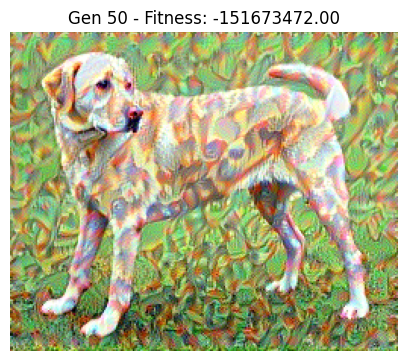
\includegraphics[width=\linewidth]{elite1.png}
    \caption{Slika za varijantu elite}
\end{subfigure}
\hfill
\begin{subfigure}{0.4\textwidth}
    \centering
    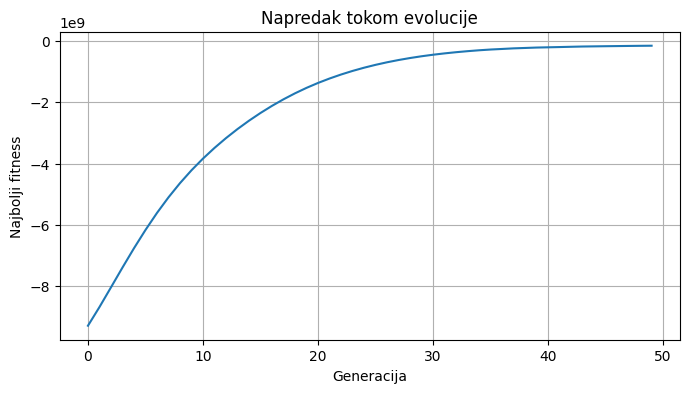
\includegraphics[width=\linewidth]{elite1gr.png}
    \caption{Grafik za varijantu elite}
\end{subfigure}

\vspace{0.1cm} % razmak između redova

\begin{subfigure}{0.4\textwidth}
    \centering
    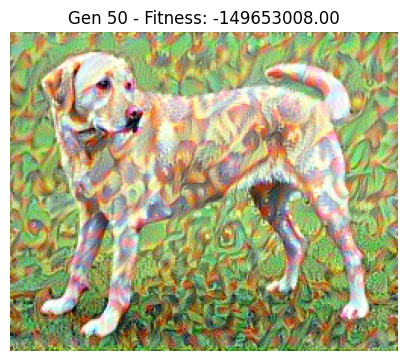
\includegraphics[width=\linewidth]{all1.png}
    \caption{Slika za varijantu all}
\end{subfigure}
\hfill
\begin{subfigure}{0.4\textwidth}
    \centering
    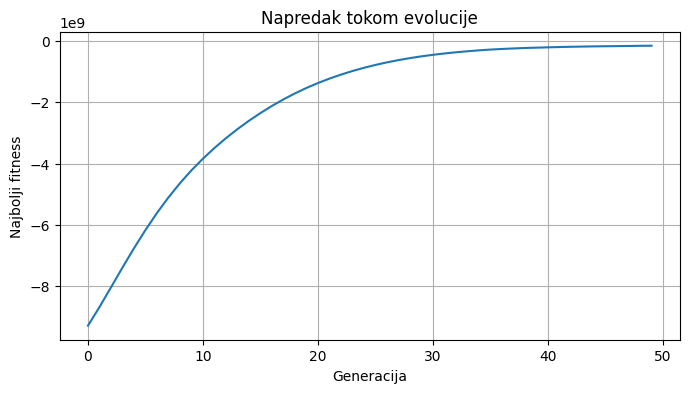
\includegraphics[width=\linewidth]{all1gr.png}
    \caption{Grafik za varijantu all}
\end{subfigure}

\caption{Uporedni prikaz rezultata i grafova za hibridni genetski algoritam: gornji red prikazuje varijantu elite, a donji red varijantu all.}
\end{figure}


\paragraph{Rezultati za $\eta_{\text{lokalno}} = 0.2$:}
\begin{itemize}
\item \textbf{Hibrid (elite):} Najbolji fitness posle 50 generacija bio je \boldmath$-7.5530 \times 10^9$\unboldmath; (gubitak $\sim 7.55\times 10^9$). Ovo predstavlja znatno lošiji rezultat nego za $\eta=0.002$. Vreme izvršavanja iznosilo je \textbf{141.15 s} (slično kao elitni 0.002 slučaj, jer je broj operacija isti).
\item \textbf{Hibrid (all):} Najbolji fitness bio je \boldmath$-6.6462 \times 10^9$\unboldmath; (gubitak $\sim 6.65\times 10^9$). Ovo je malo bolje od "elite" varijante, ali i dalje znatno lošije od rezultata postignutih sa malom $\eta$. Vreme izvršavanja iznosilo je \textbf{309.94 s} (dvostruko sporije zbog lokalne pretrage na celoj populaciji).
\end{itemize}
Rezultati su na prvi pogled iznenađujući: očekivalo se da veća lokalna stopa (agresivniji Adam) brže smanjuje gubitak. Međutim, najbolje jedinke su zaglavile na znatno lošijim vrednostima. Analiza ponašanja otkrila je \textbf{nestabilnost} evolucije kada je lokalna pretraga previše jaka. Grafik najboljeg fitnessa po generacijama (Slika 4) za $\eta=0.2$ pokazuje oscilatorno ponašanje i velike skokove: u nekim generacijama fitness naglo skoči (gubitak se smanji), dok u sledećoj može opasti. To se dešava jer preagresivna optimizacija za samo 2 koraka može pregaziti dobro rešenje i odvesti jedinku u lošiji region rešenja (npr. overshooting u optimizaciji). Posebno u slučaju "elite", gde se u svakoj generaciji dotiču samo najbolje jedinke, može se desiti da najbolja jedinka posle lokalne pretrage zapravo postane lošija (poveća joj se gubitak) usled prevelikog koraka, ali nema redundancije jer se radi samo na 2 jedinke. U varijanti "all", situacija je malo ublažena jer se više jedinki paralelno pretražuje, pa postoji veća šansa da bar neka ostane ili postane bolja. Zato "all", sa 0.2 daje nešto bolji fitness od "elite", sa 0.2 na kraju. Ipak, obe su daleko iza rezultata sa manjom stopom. Zaključak je da \textbf{preveliki lokalni koraci mogu destabilizovati evoluciju i odvesti proces u suboptimalne tokove}. GA generiše raznolika rešenja, ali ih Adam suviše grubo modifikuje i može uništiti dobru kombinatoriku u pikselskim odnosima, dovodeći do većeg gubitka. Manja stopa omogućava postupne, sigurne popravke bez overshoot-a.

\begin{figure}[h]
\centering
\begin{subfigure}{0.4\textwidth}
    \centering
    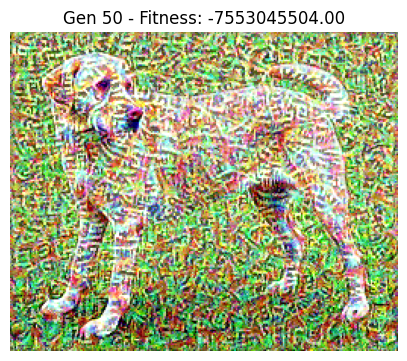
\includegraphics[width=\linewidth]{elite2.png}
    \caption{Slika za varijantu elite}
\end{subfigure}
\hfill
\begin{subfigure}{0.4\textwidth}
    \centering
    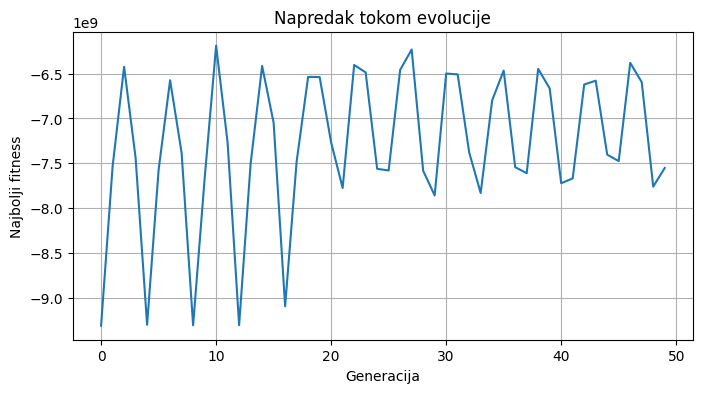
\includegraphics[width=\linewidth]{elite2gr.png}
    \caption{Grafik za varijantu elite}
\end{subfigure}

\vspace{0.1cm} % razmak između redova

\begin{subfigure}{0.4\textwidth}
    \centering
    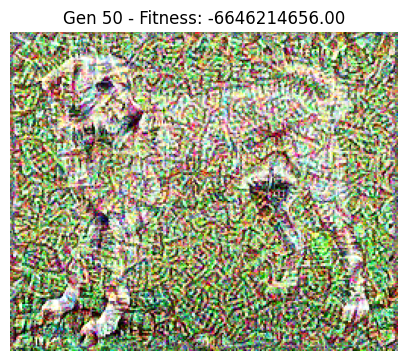
\includegraphics[width=\linewidth]{all2.png}
    \caption{Slika za varijantu all}
\end{subfigure}
\hfill
\begin{subfigure}{0.4\textwidth}
    \centering
    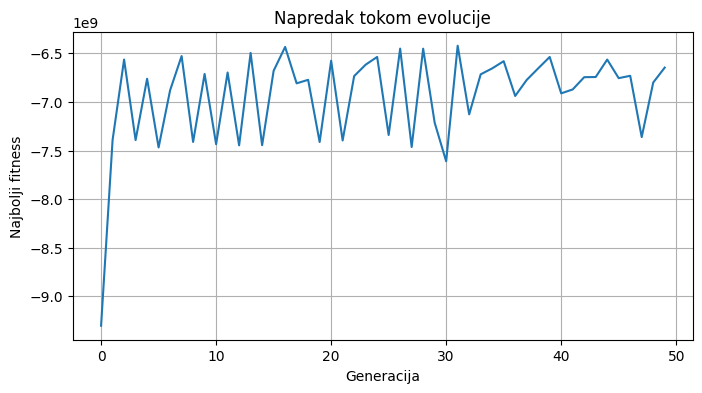
\includegraphics[width=\linewidth]{all2gr.png}
    \caption{Grafik za varijantu all}
\end{subfigure}

\caption{Uporedni prikaz rezultata i grafova za hibridni genetski algoritam: gornji red prikazuje varijantu elite, a donji red varijantu all.}
\end{figure}

\newpage

\paragraph{Rezultati za $\eta_{\text{lokalno}} = 0.02$ (elitni slučaj):}
Kao kompromis, isprobana je još jedna vrednost stope, $0.02$, samo za \texttt{apply\_local\_to="elite"} (jer se utvrdilo da "all" nepotrebno troši vreme bez boljitka za male korake). Dobijeni najbolji fitness bio je \boldmath$-1.9651 \times 10^8$\unboldmath; (gubitak $\sim 1.965\times10^8$). Ovo je nešto lošije od rezultata sa 0.002 (-1.5167e8), ali ne drastično. Posmatrajući krivu u funkciji generacija, uočeno je da je \textbf{već do 10. generacije fitness dostigao vrlo dobru vrednost (blizu konačne)}, nakon čega je uglavnom oscilovao blago oko tog nivoa, bez značajne opadajuće putanje kao kod 0.002. To sugeriše da je $\eta=0.02$ bila dovoljno velika da brzo dovede najbolju jedinku blizu nekog optimuma, ali da je nakon toga možda uvodila male nestabilnosti (jedinka je skakala oko te vrednosti umesto da se usporeno približava daljem minimumu). Vreme izvršavanja za ovaj slučaj iznosilo je \textbf{150.91 s}, praktično isto kao i za 0.002, što se i očekivalo (operacije su iste vrste i količine).

\begin{figure}[h]
\centering
\begin{minipage}[b]{0.48\textwidth}
    \centering
    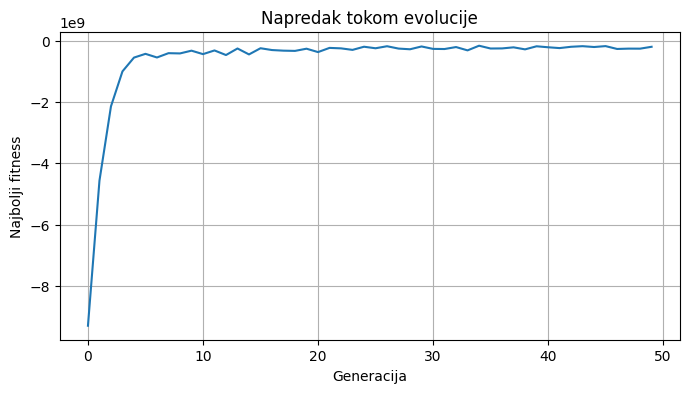
\includegraphics[width=\textwidth]{elite3gr.png} 
    \caption*{Fitness kriva}
\end{minipage}
\hfill
\begin{minipage}[b]{0.48\textwidth}
    \centering
    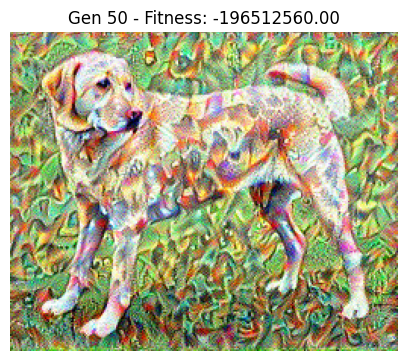
\includegraphics[width=\textwidth]{elite3.png} 
    \caption*{Konačna slika}
\end{minipage}
\caption{$\eta_{\text{lokalno}}=0.02$ (elitni slučaj)}
\end{figure}


\subsection{Poređenje svih metoda i diskusija rezultata}
Na kraju, upoređeni su svi dobijeni rezultati: bazni Adam pristup, čisti GA i hibridne GA varijante. U tabeli~1 navedeni su najbolji postignuti fitness (i odgovarajući gubitak) i vreme izvođenja za svaku testiranu konfiguraciju.

\begin{table}[h]
\centering
\begin{tabular}{l|c|c}
\hline
Metod & Najbolji fitness (posle 50 gen/1000 koraka) & Vreme (s) \\
\hline
Adam (bazni NST, 1000 koraka) & -- ($L_{\text{ukupno}} \approx 1.28 \times 10^7$) & 23.2 \\
GA bez lokalne pretrage & $-9.2524 \times 10^9$ & 118.13 \\
GA hibrid (elite, $\eta=0.002$) & $-1.5167 \times 10^8$ & 140.72 \\
GA hibrid (all, $\eta=0.002$) & $-1.4965 \times 10^8$ & 308.22 \\
GA hibrid (elite, $\eta=0.2$) & $-7.5530 \times 10^9$ & 141.15 \\
GA hibrid (all, $\eta=0.2$) & $-6.6462 \times 10^9$ & 309.94 \\
GA hibrid (elite, $\eta=0.02$) & $-1.9651 \times 10^8$ & 150.91 \\
\hline
\end{tabular}
\caption{Poređenje rezultata različitih pristupa.}
\end{table}

\newpage
Iz tabele su odmah uočljivi sledeći zaključci:
\begin{itemize}
\item \textbf{Bazni Adam optimizator daje ubedljivo najbolji rezultat i najbrži je.} Nakon 1000 iteracija (23.2 s) postignut je $L\approx1.28\times10^7$, što nijedna GA varijanta nije ni približno dostigla ni za duži vremenski period. Kvalitativno, slika dobijena ovim pristupom bila je vizuelno najoštrija i najprihvatljivija (jasno se prepoznaje sadržaj, a stil je prenet u finim detaljima).
\item \textbf{Čisti GA (bez lokalne pretrage) je praktično neuspešan} za realnu stilizaciju. Fitness $-9.25\times10^9$ znači $L\approx9.25\times10^9$, što je tri reda veličine gore od Adam rešenja. Takva slika jedva da liči na stilizovanu – vrlo bliska sadržajnoj slici sa minimalnim tragovima stila (jer je populacija inicijalizovana sadržajnom slikom i pomerala se minimalno). Dakle, evolutivni operatori sami po sebi nisu uspeli da dovoljno adaptiraju sliku ka stilu kroz 50 generacija.
\item \textbf{Dodavanje lokalne pretrage (hibridni GA) drastično poboljšava rezultat} u odnosu na čisti GA. Najbolje vrednosti gubitka pale su na red $10^8$, što je oko 50–60 puta manje nego kod čistog GA. To potvrđuje da gradijentni koraci unutar evolucije obavljaju najveći deo posla u smislu prilagođavanja slike. Vrednosti gubitka su reda $1\times10^8$, što je i dalje oko 10 puta više nego kod samog Adam optimizatora.
\item \textbf{Poređenje "elite" vs "all":} Za malu stopu ($0.002$) pokazalo se da "all" ne donosi gotovo ništa u pogledu kvaliteta konačne slike u odnosu na "elite", a vreme eksponencijalno raste. Za veću stopu ($0.2$) "all" je dao nešto bolji rezultat od "elite", što sugeriše da u nestabilnijim uslovima postoji korist od paralelne eksploatacije više jedinki (neke će postići bolje rezultate od drugih). Međutim, rezultati su generalno slabi. Dakle, ako se koristi hibridni pristup, \textbf{bolje je lokalno pretraživati samo nekoliko najboljih jedinki} kako bi se uštedelo vreme i sačuvala diverzitet populacije (u "all", slučaju svi se pretvaraju u slična lokalno-optimizovana rešenja, što može smanjiti raznolikost populacije).
\item \textbf{Uticaj stope lokalnog učenja:} Premala vrednost ($0.002$) bila je sigurna i efektivna, dok je prevelika ($0.2$) bila kontraproduktivna. Srednja vrednost ($0.02$) dala je bržu inicijalnu konvergenciju, ali je zaglavljena blizu rezultata male stope. Moguće je da bi još niži $\eta$ od $0.002$ doveo do manjeg konačnog gubitka, ali bi to zahtevalo mnogo više generacija. Veći broj lokalnih koraka $m$ bi poboljšao rezultate, približavajući ih direktnom Adam rešenju. U ekstremu, vrlo veliki broj $m$ pretvorio bi hibridni algoritam u višestruko pokretanje Adam optimizacije iz različitih nasumičnih inicijalizacija, pri čemu bi sve verovatno konvergiralo na slično rešenje (s obzirom da su inicijalno sve slike bliske sadržajnoj slici).
\end{itemize}

\paragraph{Završna diskusija:} Serija eksperimenata pokazuje da klasični pristup neuronskom prenosu stila (direktna optimizacija piksela gradijentom) nadmašuje evolutivni pristup u pogledu kvaliteta rešenja i brzine. Genetski algoritam, čak i uz određenu pomoć gradijentnih mutacija, bez dodatne lokalne pretrage nije uspeo efikasno da optimizuje sliku. Dodavanje lokalne pretrage (Adam koraka) u genetski algoritam značajno poboljšava rezultate, što ukazuje da gradijent obavlja najvažniji deo posla u podešavanju slike, dok GA služi za pružanje različitih početnih stanja i globalnu pretragu. U ovom slučaju svi članovi populacije su počinjali slično (oko sadržajne slike), pa je diverzitet populacije bio ograničen; bolji efekti GA bi se mogli videti kod raznovrsnijih inicijalizacija (npr. nasumične slike, različite kombinacije sadržaja i stila). S obzirom na ekstremnu dimenzionalnost problema, evolucioni algoritam bi zahtevao mnogo veće populacije i mnogo generacija da se približi efektu jednog gradijentnog spusta, što postaje nepraktično.

Jedan scenario u kojem bi GA mogao imati prednost su slučajevi sa nediferencijabilnom funkcijom cilja ili dodatno diskretizovanim ograničenjima. Na primer, ako bi se generisana slika sastojala od diskretnih elemenata ili ograničenog skupa boja, gradijentni metod se ne bi mogao direktno primeniti, pa bi evolucioni pristup imao smisla. U čistom NST problemu, diferencijabilnost i snažna orijentacija gradijenta ka minimumu daje preveliku prednost gradijentskoj optimizaciji.

\section{Zaključak}
U ovom projektu implementiran je neuronski prenos stila koristeći VGG19 mrežu za izdvajanje karakteristika sadržaja i stila, i ispitana su dva različita optimizaciona pristupa: direktni gradijentski (Adam) i populacioni evolucioni (genetski algoritam), kao i njihova kombinacija. Detaljno je analizirana uloga svakog dela algoritma (od grafa duboke mreže i Gramove matrice do operatora GA i hibridne lokalne pretrage) kako bi se razumelo zašto neki pristupi daju bolje rezultate.

Eksperimentalni rezultati jasno pokazuju da je za problem neuralnog prenosa stila gradijentna optimizacija mnogo efikasnija i efektivnija od genetske evolucije. Adam optimizator je u kratkom vremenu dao najbolje rešenje (najniži gubitak i vizuelno najbolju sliku). Osnovni genetski algoritam napredovao je sporo i zapinjao na rešenjima daleko od optimuma. Integracijom lokalnih Adam koraka unutar GA poboljšan je evolucioni pristup, ali svaka jedinka praktično funkcioniše kao zasebna NST optimizacija, što u limitu odgovara višestrukom pokretanju Adam algoritma. Hibridni pristup nije dostigao kvalitet baznog Adam rezultata u datom broju iteracija i zahtevao je više računske snage.

Zaključuje se da, za kontinuirani optimizacioni problem kao što je stilizacija slike, gradijentne metode ostaju metoda izbora. Genetski algoritam može imati edukativnu vrednost i eventualno pružiti raznolika rešenja (npr. više različitih stilizacija), ali u pogledu optimizacije same funkcije gubitka on je inferioran. Hibridni pristup može spojiti prednosti oba sveta, ali najveći teret posla i dalje nose gradijentski koraci.

U budućim radovima može se ispitati da li evolucioni algoritmi imaju prednost u nekim varijantama zadatka prenosa stila – npr. kada su definisani kriterijumi koji nisu glatki niti diferencijabilni (prilagođavanje stila ljudskoj oceni ili diskretnim umetničkim pravilima). Takođe, može se razmotriti korišćenje drugih globalnih optimizacionih metoda (poput simuliranog kaljenja, roja čestica itd.) za poređenje, kao i upotreba unapred istreniranih modela za direktno generisanje stilizovanih slika (moderni feed-forward NST modeli) trenirani na mnogim iteracijama gradijentnog spusta, a zatim sposobni da izvrše prenos stila jednim prolazom.

\newpage

\begin{thebibliography}{99}

\bibitem{Gatys2015}
Leon A. Gatys, Alexander S. Ecker, Matthias Bethge. 
\textit{A Neural Algorithm of Artistic Style}.\\
Dostupno na: \href{https://arxiv.org/abs/1508.06576}{https://arxiv.org/abs/1508.06576}

\bibitem{WikipediaNST}
Neural Style Transfer — Wikipedia.\\
Dostupno na: \href{https://en.wikipedia.org/wiki/Neural_style_transfer}{https://en.wikipedia.org/wiki/Neural\_style\_transfer}

\bibitem{Bruyere2021}
Bruyère, “Creativity in Artificial Intelligence: Creating artworks using Evolutionary Algorithms for Style Transfer”, 2021.\\
Dostupno na: \href{https://www.researchgate.net/publication/355859299_Creativity_in_Artificial_Intelligence_Creating_artworks_using_Evolutionary_Algorithms_for_Style_Transfer}{https://www.researchgate.net/publication/355859299\_Creativity\_in\_Artificial\_Intelligence\_Creating\_artworks\_using\_Evolutionary\_Algorithms\_for\_Style\_Transfer}

\bibitem{D2L2021}
Dive into Deep Learning (D2L), Section 14.12 — Neural Style Transfer.\\
Dostupno na: \href{http://d2l.ai/chapter_computer-vision/neural-style.html}{http://d2l.ai/chapter\_computer-vision/neural-style.html}

\bibitem{TensorFlowNST}
TensorFlow Tutorials — Neural Style Transfer.\\
Dostupno na: \href{https://www.tensorflow.org/tutorials/generative/style_transfer}{https://www.tensorflow.org/tutorials/generative/style\_transfer}

\end{thebibliography}


\end{document}
